\documentclass[8pt,ignorenonframetext,dvipsnames]{beamer}
\setbeamertemplate{caption}[numbered]
\setbeamertemplate{caption label separator}{: }
\setbeamercolor{caption name}{fg=normal text.fg}
\beamertemplatenavigationsymbolsempty
\usepackage{lmodern}
\usepackage{amssymb,amsmath}
\usepackage{ifxetex,ifluatex}
\usepackage{fixltx2e} % provides \textsubscript
\ifnum 0\ifxetex 1\fi\ifluatex 1\fi=0 % if pdftex
  \usepackage[T1]{fontenc}
  \usepackage[utf8]{inputenc}
\else % if luatex or xelatex
  \ifxetex
    \usepackage{mathspec}
  \else
    \usepackage{fontspec}
  \fi
  \defaultfontfeatures{Ligatures=TeX,Scale=MatchLowercase}
\fi
% use upquote if available, for straight quotes in verbatim environments
\IfFileExists{upquote.sty}{\usepackage{upquote}}{}
% use microtype if available
\IfFileExists{microtype.sty}{%
\usepackage{microtype}
\UseMicrotypeSet[protrusion]{basicmath} % disable protrusion for tt fonts
}{}
\newif\ifbibliography
\hypersetup{
            pdftitle={Managing and Manipulating Data Using R},
            pdfauthor={Patricia Martin},
            pdfborder={0 0 0},
            breaklinks=true}
\urlstyle{same}  % don't use monospace font for urls
\usepackage{color}
\usepackage{fancyvrb}
\newcommand{\VerbBar}{|}
\newcommand{\VERB}{\Verb[commandchars=\\\{\}]}
\DefineVerbatimEnvironment{Highlighting}{Verbatim}{commandchars=\\\{\}}
% Add ',fontsize=\small' for more characters per line
\usepackage{framed}
\definecolor{shadecolor}{RGB}{248,248,248}
\newenvironment{Shaded}{\begin{snugshade}}{\end{snugshade}}
\newcommand{\KeywordTok}[1]{\textcolor[rgb]{0.13,0.29,0.53}{\textbf{#1}}}
\newcommand{\DataTypeTok}[1]{\textcolor[rgb]{0.13,0.29,0.53}{#1}}
\newcommand{\DecValTok}[1]{\textcolor[rgb]{0.00,0.00,0.81}{#1}}
\newcommand{\BaseNTok}[1]{\textcolor[rgb]{0.00,0.00,0.81}{#1}}
\newcommand{\FloatTok}[1]{\textcolor[rgb]{0.00,0.00,0.81}{#1}}
\newcommand{\ConstantTok}[1]{\textcolor[rgb]{0.00,0.00,0.00}{#1}}
\newcommand{\CharTok}[1]{\textcolor[rgb]{0.31,0.60,0.02}{#1}}
\newcommand{\SpecialCharTok}[1]{\textcolor[rgb]{0.00,0.00,0.00}{#1}}
\newcommand{\StringTok}[1]{\textcolor[rgb]{0.31,0.60,0.02}{#1}}
\newcommand{\VerbatimStringTok}[1]{\textcolor[rgb]{0.31,0.60,0.02}{#1}}
\newcommand{\SpecialStringTok}[1]{\textcolor[rgb]{0.31,0.60,0.02}{#1}}
\newcommand{\ImportTok}[1]{#1}
\newcommand{\CommentTok}[1]{\textcolor[rgb]{0.56,0.35,0.01}{\textit{#1}}}
\newcommand{\DocumentationTok}[1]{\textcolor[rgb]{0.56,0.35,0.01}{\textbf{\textit{#1}}}}
\newcommand{\AnnotationTok}[1]{\textcolor[rgb]{0.56,0.35,0.01}{\textbf{\textit{#1}}}}
\newcommand{\CommentVarTok}[1]{\textcolor[rgb]{0.56,0.35,0.01}{\textbf{\textit{#1}}}}
\newcommand{\OtherTok}[1]{\textcolor[rgb]{0.56,0.35,0.01}{#1}}
\newcommand{\FunctionTok}[1]{\textcolor[rgb]{0.00,0.00,0.00}{#1}}
\newcommand{\VariableTok}[1]{\textcolor[rgb]{0.00,0.00,0.00}{#1}}
\newcommand{\ControlFlowTok}[1]{\textcolor[rgb]{0.13,0.29,0.53}{\textbf{#1}}}
\newcommand{\OperatorTok}[1]{\textcolor[rgb]{0.81,0.36,0.00}{\textbf{#1}}}
\newcommand{\BuiltInTok}[1]{#1}
\newcommand{\ExtensionTok}[1]{#1}
\newcommand{\PreprocessorTok}[1]{\textcolor[rgb]{0.56,0.35,0.01}{\textit{#1}}}
\newcommand{\AttributeTok}[1]{\textcolor[rgb]{0.77,0.63,0.00}{#1}}
\newcommand{\RegionMarkerTok}[1]{#1}
\newcommand{\InformationTok}[1]{\textcolor[rgb]{0.56,0.35,0.01}{\textbf{\textit{#1}}}}
\newcommand{\WarningTok}[1]{\textcolor[rgb]{0.56,0.35,0.01}{\textbf{\textit{#1}}}}
\newcommand{\AlertTok}[1]{\textcolor[rgb]{0.94,0.16,0.16}{#1}}
\newcommand{\ErrorTok}[1]{\textcolor[rgb]{0.64,0.00,0.00}{\textbf{#1}}}
\newcommand{\NormalTok}[1]{#1}
\usepackage{longtable,booktabs}
\usepackage{caption}
% These lines are needed to make table captions work with longtable:
\makeatletter
\def\fnum@table{\tablename~\thetable}
\makeatother
\usepackage{graphicx,grffile}
\makeatletter
\def\maxwidth{\ifdim\Gin@nat@width>\linewidth\linewidth\else\Gin@nat@width\fi}
\def\maxheight{\ifdim\Gin@nat@height>\textheight0.8\textheight\else\Gin@nat@height\fi}
\makeatother
% Scale images if necessary, so that they will not overflow the page
% margins by default, and it is still possible to overwrite the defaults
% using explicit options in \includegraphics[width, height, ...]{}
\setkeys{Gin}{width=\maxwidth,height=\maxheight,keepaspectratio}

% Prevent slide breaks in the middle of a paragraph:
\widowpenalties 1 10000
\raggedbottom

\AtBeginPart{
  \let\insertpartnumber\relax
  \let\partname\relax
  \frame{\partpage}
}
\AtBeginSection{
  \ifbibliography
  \else
    \let\insertsectionnumber\relax
    \let\sectionname\relax
    \frame{\sectionpage}
  \fi
}
\AtBeginSubsection{
  \let\insertsubsectionnumber\relax
  \let\subsectionname\relax
  \frame{\subsectionpage}
}

\setlength{\parindent}{0pt}
\setlength{\parskip}{6pt plus 2pt minus 1pt}
\setlength{\emergencystretch}{3em}  % prevent overfull lines
\providecommand{\tightlist}{%
  \setlength{\itemsep}{0pt}\setlength{\parskip}{0pt}}
\setcounter{secnumdepth}{0}

%packages
\usepackage{graphicx}
\usepackage{rotating}
\usepackage{hyperref}

\usepackage{tikz} % used for text highlighting, amongst others
%title slide stuff
%\institute{Department of Education}
%\title{Managing and Manipulating Data Using R}

%
\setbeamertemplate{navigation symbols}{} % get rid of navigation icons:

%\setbeamertemplate{frametitle}{\thesection \hspace{0.2cm} \insertframetitle}
\setbeamertemplate{section in toc}[sections numbered]
\setbeamertemplate{subsection in toc}[subsections numbered]

%define colors
%\definecolor{uva_orange}{RGB}{216,141,42} % UVa orange (Rotunda orange)
\definecolor{mygray}{rgb}{0.95, 0.95, 0.95} % for highlighted text
	% grey is equal parts red, green, blue. higher values >> lighter grey
	%\definecolor{lightgraybo}{rgb}{0.83, 0.83, 0.83}

% new commands

%highlight text with very light grey
\newcommand*{\hlg}[1]{%
	\tikz[baseline=(X.base)] \node[rectangle, fill=mygray] (X) {#1};%
}
%, inner sep=0.3mm
%highlight text with very light grey and use font associated with code
\newcommand*{\hlgc}[1]{\texttt{\hlg{#1}}}

% Font
\usepackage[defaultfam,light,tabular,lining]{montserrat}
\usepackage[T1]{fontenc}
\renewcommand*\oldstylenums[1]{{\fontfamily{Montserrat-TOsF}\selectfont #1}}

% Change color of boldface text to darkgray
\renewcommand{\textbf}[1]{{\color{darkgray}\bfseries\fontfamily{Montserrat-TOsF}#1}}

% Bullet points
\setbeamertemplate{itemize item}{\color{BlueViolet}$\circ$}
\setbeamertemplate{itemize subitem}{\color{BrickRed}$\triangleright$}
\setbeamertemplate{itemize subsubitem}{$-$}

% Reduce space before lists
\addtobeamertemplate{itemize/enumerate body begin}{}{\vspace*{-8pt}}

\title{Managing and Manipulating Data Using R}
\subtitle{Lecture 8, Acquiring data in R}
\author{Patricia Martin}
\date{}

\begin{document}
\frame{\titlepage}

\begin{frame}
\tableofcontents[hideallsubsections]
\end{frame}

\section{Introduction}\label{introduction}

\begin{frame}[fragile]{Libraries we will use today {[}install if you
don't have them{]}}

\begin{Shaded}
\begin{Highlighting}[]
\KeywordTok{library}\NormalTok{(dplyr)}
\KeywordTok{library}\NormalTok{(readr)}
\KeywordTok{library}\NormalTok{(haven)}
\KeywordTok{library}\NormalTok{(readxl)}
\KeywordTok{library}\NormalTok{(labelled)}
\end{Highlighting}
\end{Shaded}

\end{frame}

\begin{frame}{Data we will use today}

\begin{itemize}
\tightlist
\item
  Integrated Postsecondary Education Data System (IPEDS)\\
\item
  High School Longitudinal Surveys (HSLS)\\
\item
  Federal Student Aid Data\\
\item
  Equality of Opportunity Project
\end{itemize}

\end{frame}

\begin{frame}{Integrated Postsecondary Education Data System (IPEDS)}

\begin{itemize}
\tightlist
\item
  Postsecondary education data from NCES\\
\item
  There are
  \href{https://nces.ed.gov/ipeds/resource/download/IPEDS_DataReleaseProcedures.pdf}{12
  survey components} and 3 collection periods
\end{itemize}

We will be working with
\href{https://nces.ed.gov/ipeds/datacenter/DataFiles.aspx}{Institutional
Characteristics data of 2017}

\end{frame}

\begin{frame}{High school longitudinal surveys from National Center for
Education Statistics (NCES)}

\begin{itemize}
\tightlist
\item
  Follow U.S. students from high school through college, labor market
\end{itemize}

We will be working with
\href{https://nces.ed.gov/surveys/hsls09/index.asp}{High School
Longitudinal Study of 2009 (HSLS:09)}

\begin{itemize}
\tightlist
\item
  Follows 9th graders from 2009
\item
  Data collection waves

  \begin{itemize}
  \tightlist
  \item
    Base Year (2009)
  \item
    First Follow-up (2012)
  \item
    2013 Update (2013)
  \item
    High School Transcripts (2013-2014)
  \item
    Second Follow-up (2016)
  \end{itemize}
\end{itemize}

\end{frame}

\begin{frame}{Federal Student Aid}

\begin{itemize}
\tightlist
\item
  Federal Student Aid Data Center provides information for federal
  assistance programs and is divided into four categories:

  \begin{itemize}
  \tightlist
  \item
    Student Aid Data\\
  \item
    School Data\\
  \item
    Federal Family Education Loan (FFEL) Program\\
  \item
    Business Information Resources
  \end{itemize}
\end{itemize}

We will be working with
\href{https://studentaid.ed.gov/sa/node/105}{School Data}

\end{frame}

\begin{frame}{Equality of Opportunity Project}

\begin{itemize}
\tightlist
\item
  \href{http://www.equality-of-opportunity.org/papers/coll_mrc_paper.pdf}{Equality
  of Opportunity Project} uses two data sources-- federal tax recoards
  and Department of Education records (1999-2013)-- to investigate
  intergenerational income mobility at colleges in the US.
\end{itemize}

We will use
\href{http://www.equality-of-opportunity.org/documents/}{Mobility Report
Cards: The Role of Colleges in Intergenerational Mobility data}

\textbf{Not sure if to simply list datasets. Lecture will go over
acquiring data and not so much about manipulating data. Not sure if
students need to know each dataset in detail?}

\end{frame}

\section{Common data formats}\label{common-data-formats}

\begin{frame}{Common data formats}

\begin{itemize}
\tightlist
\item
  Comma-separated values (.csv)\\
\item
  Excel (.xls or .xlsx)\\
\item
  Text-formated data (.txt)\\
\item
  Tab-separated values (.tsv)
\item
  R (.Rdata or .rds)\\
\item
  Stata (.dta)
\item
  SPSS (.sav)\\
\item
  SAS (.sas)
\end{itemize}

\end{frame}

\section{\texorpdfstring{\texttt{readr}
package}{readr package}}\label{readr-package}

\begin{frame}[fragile]{\texttt{readr}}

The \href{https://readr.tidyverse.org/index.html}{\texttt{readr}}
package is part of tidyverse, which is designed to read in flat data
files in R and transform them into data frames.\\[2\baselineskip]- We
could load \textbf{library(tidyverse)} if we wanted to load all packages
in tidyverse (e.g.~ggplot2, dplyr, tidyr, stringr, readr, etc\ldots{})

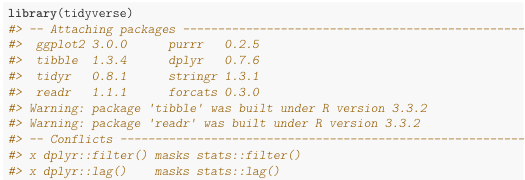
\includegraphics{~/Desktop/GitHub/rclass/lectures/lecture8/tidyverse.png}\\
- For the purpose of this lecture, we will just need to load
\textbf{library(readr)}

\end{frame}

\begin{frame}[fragile]{\texttt{readr}}

No matter the flat file format you are working with, there are two
important steps for reading in data with \texttt{readr}:

\begin{enumerate}
\def\labelenumi{(\arabic{enumi})}
\item
  \textbf{a function to parse the file (read\_csv)}
\item
  \textbf{column specification}
\end{enumerate}

\end{frame}

\begin{frame}[fragile]{\texttt{readr\ functions}}

\textbf{readr's} (tidyverse) functions

\begin{longtable}[]{@{}ll@{}}
\toprule
\textbf{Format} & \textbf{Function}\tabularnewline
\midrule
\endhead
Comma-separated values (csv) & \texttt{read\_csv}\tabularnewline
Semicolon separated files & \texttt{read\_csv2}\tabularnewline
Tab-separated values (tsv) & \texttt{read\_tsv}\tabularnewline
Any delimiter & \texttt{read\_delim}\tabularnewline
Fixed width files & \texttt{read\_fwf}\tabularnewline
Text-formated data (txt) & \texttt{read\_table}\tabularnewline
Web log files & \texttt{read\_log}\tabularnewline
\bottomrule
\end{longtable}

\end{frame}

\begin{frame}[fragile]{\texttt{readr\ column\ specification}}

\texttt{readr} is pretty good at guessing each column's data type
(e.g.~character, double, etc.), however it is good practice to manually
specify the data type for each column.

\begin{Shaded}
\begin{Highlighting}[]
\NormalTok{mtcars <-}\StringTok{ }\KeywordTok{read_csv}\NormalTok{(}\KeywordTok{readr_example}\NormalTok{(}\StringTok{"mtcars.csv"}\NormalTok{))}
\CommentTok{#> Parsed with column specification:}
\CommentTok{#> cols(}
\CommentTok{#>   mpg = col_double(),}
\CommentTok{#>   cyl = col_integer(),}
\CommentTok{#>   disp = col_double(),}
\CommentTok{#>   hp = col_integer(),}
\CommentTok{#>   drat = col_double(),}
\CommentTok{#>   wt = col_double(),}
\CommentTok{#>   qsec = col_double(),}
\CommentTok{#>   vs = col_integer(),}
\CommentTok{#>   am = col_integer(),}
\CommentTok{#>   gear = col_integer(),}
\CommentTok{#>   carb = col_integer()}
\CommentTok{#> )}
\end{Highlighting}
\end{Shaded}

\end{frame}

\begin{frame}[fragile]{\texttt{readr\ column\ specification}}

The output of the previous example shows us the column specification
readr gave us. However, we could manually change column specification if
we do not like readr's guess.

\begin{Shaded}
\begin{Highlighting}[]
\NormalTok{mtcars <-}\StringTok{ }\KeywordTok{read_csv}\NormalTok{(}\KeywordTok{readr_example}\NormalTok{(}\StringTok{"mtcars.csv"}\NormalTok{), }\DataTypeTok{col_types =} 
  \KeywordTok{cols}\NormalTok{(}
    \DataTypeTok{mpg =} \KeywordTok{col_double}\NormalTok{(),}
    \DataTypeTok{cyl =} \KeywordTok{col_integer}\NormalTok{(),}
    \DataTypeTok{disp =} \KeywordTok{col_double}\NormalTok{(),}
    \DataTypeTok{hp =} \KeywordTok{col_integer}\NormalTok{(),}
    \DataTypeTok{drat =} \KeywordTok{col_double}\NormalTok{(),}
    \DataTypeTok{vs =} \KeywordTok{col_integer}\NormalTok{(),}
    \DataTypeTok{wt =} \KeywordTok{col_double}\NormalTok{(),}
    \DataTypeTok{qsec =} \KeywordTok{col_double}\NormalTok{(),}
    \DataTypeTok{am =} \KeywordTok{col_integer}\NormalTok{(),}
    \DataTypeTok{gear =} \KeywordTok{col_integer}\NormalTok{(),}
    \DataTypeTok{carb =} \KeywordTok{col_integer}\NormalTok{()}
\NormalTok{  )}
\NormalTok{)}
\end{Highlighting}
\end{Shaded}

\end{frame}

\begin{frame}[fragile]{\texttt{readr} features}

\begin{itemize}
\tightlist
\item
  \textbf{skip}: \texttt{read\_csv}(csv file, skip = n)\\
\item
  \textbf{comment}: \texttt{read\_csv}(csv file, comment = ``\#'')\\
\item
  \textbf{col\_names}: \texttt{read\_csv}(csv file, col\_names =
  c(``x'', ``y'', ``z''))
\end{itemize}

\end{frame}

\begin{frame}[fragile]{\texttt{readr} demonstration csv}

\texttt{readr} automatically treats the first line of data as column
names.

\begin{Shaded}
\begin{Highlighting}[]
\KeywordTok{read_csv}\NormalTok{(}\StringTok{"column 1, column 2, column 3}
\StringTok{         1,2,3}
\StringTok{         4,5,6"}
\NormalTok{         )}
\CommentTok{#> # A tibble: 2 x 3}
\CommentTok{#>   `column 1` `column 2` `column 3`}
\CommentTok{#>        <int>      <int>      <int>}
\CommentTok{#> 1          1          2          3}
\CommentTok{#> 2          4          5          6}
\end{Highlighting}
\end{Shaded}

There are instances where you may want to tell R from what line to begin
reading in data.

\end{frame}

\begin{frame}[fragile]{\texttt{readr} demonstration csv}

Notice the example below. The first two lines are comments about the
data. We would need to use \textbf{skip = n} to skip n lines.

\begin{Shaded}
\begin{Highlighting}[]
\KeywordTok{read_csv}\NormalTok{(}\StringTok{"This file contains data on student charges for the acdemic year.}
\StringTok{         File name: IC2016_AY}
\StringTok{         a, b, c}
\StringTok{         1,2,3}
\StringTok{         4,5,6"}\NormalTok{, }\DataTypeTok{skip =} \DecValTok{2}
\NormalTok{         )}
\CommentTok{#> # A tibble: 2 x 3}
\CommentTok{#>       a     b     c}
\CommentTok{#>   <int> <int> <int>}
\CommentTok{#> 1     1     2     3}
\CommentTok{#> 2     4     5     6}
\end{Highlighting}
\end{Shaded}

\end{frame}

\begin{frame}[fragile]{\texttt{readr} demonstration csv}

We could also tell R to drop lines we specify as comments. With
\textbf{comment = n}

\begin{Shaded}
\begin{Highlighting}[]
\KeywordTok{read_csv}\NormalTok{(}\StringTok{"# This file contains data on student charges for the acdemic year.}
\StringTok{         a, b, c}
\StringTok{         1,2,3}
\StringTok{         4,5,6"}\NormalTok{, }\DataTypeTok{comment =} \StringTok{"#"}
\NormalTok{         )}
\CommentTok{#> # A tibble: 2 x 3}
\CommentTok{#>       a     b     c}
\CommentTok{#>   <int> <int> <int>}
\CommentTok{#> 1     1     2     3}
\CommentTok{#> 2     4     5     6}
\end{Highlighting}
\end{Shaded}

\begin{Shaded}
\begin{Highlighting}[]
\KeywordTok{read_csv}\NormalTok{(}\StringTok{"* This file contains data on student charges for the acdemic year.}
\StringTok{         a, b, c}
\StringTok{         1,2,3}
\StringTok{         4,5,6"}\NormalTok{, }\DataTypeTok{comment =} \StringTok{"*"}
\NormalTok{         )}
\CommentTok{#> # A tibble: 2 x 3}
\CommentTok{#>       a     b     c}
\CommentTok{#>   <int> <int> <int>}
\CommentTok{#> 1     1     2     3}
\CommentTok{#> 2     4     5     6}
\end{Highlighting}
\end{Shaded}

\end{frame}

\begin{frame}[fragile]{\texttt{readr} column names}

We could tell R there are no column names with \textbf{col\_names =
FALSE} or we could manually give R column names with \textbf{col\_names
= c(``'', ``'', ``'')}

\begin{Shaded}
\begin{Highlighting}[]
\KeywordTok{read_csv}\NormalTok{(}\StringTok{"1,2,3}
\StringTok{         4,5,6"}\NormalTok{, }\DataTypeTok{col_names =} \OtherTok{FALSE}
\NormalTok{         )}
\CommentTok{#> # A tibble: 2 x 3}
\CommentTok{#>      X1    X2    X3}
\CommentTok{#>   <int> <int> <int>}
\CommentTok{#> 1     1     2     3}
\CommentTok{#> 2     4     5     6}
\end{Highlighting}
\end{Shaded}

\begin{Shaded}
\begin{Highlighting}[]
\KeywordTok{read_csv}\NormalTok{(}\StringTok{"1,2,3}
\StringTok{         4,5,6"}\NormalTok{, }\DataTypeTok{col_names =} \KeywordTok{c}\NormalTok{(}\StringTok{"column 1"}\NormalTok{, }\StringTok{"column 2"}\NormalTok{, }\StringTok{"column 3"}\NormalTok{)}
\NormalTok{         )}
\CommentTok{#> # A tibble: 2 x 3}
\CommentTok{#>   `column 1` `column 2` `column 3`}
\CommentTok{#>        <int>      <int>      <int>}
\CommentTok{#> 1          1          2          3}
\CommentTok{#> 2          4          5          6}
\end{Highlighting}
\end{Shaded}

\end{frame}

\begin{frame}{\texttt{readr} Student exercise}

\begin{itemize}
\tightlist
\item
  Get in your homework groups\\
\item
  Create a 3x3 tibble like the examples above
  (e.g.~read\_csv(``a,b,c\ldots{}.'')), treating the first line as
  column names\\
\item
  Now on the first line add a sentence\\
\item
  This time add a special character ( *, \#, ! ) at the beginning of the
  sentence and indicate it is a comment\\
\item
  Delete the sentence and column names (should have a 2x2 tibble) and
  manually tell R column names
\end{itemize}

\end{frame}

\begin{frame}[fragile]{\texttt{readr} demonstration csv}

\textbf{NOT SURE IF TO MAKE THIS A DEMONSTRATION WHERE STUDENTS FOLLOW
ALONG OR ANOTHER STUDENT EXERCISE}\\
\textbf{Tying it all together}

Use \texttt{read\_csv()} function from \texttt{readr} to import csv
dataset into R without column specification. Follow along on your
computers.

\begin{Shaded}
\begin{Highlighting}[]
\NormalTok{ipeds <-}\StringTok{ }\KeywordTok{read_csv}\NormalTok{(}\DataTypeTok{file=}\StringTok{"~/Desktop/GitHub/rclass/data/ipeds/ic/ipeds_hd_2017_small.csv"}\NormalTok{)}
\CommentTok{#> Parsed with column specification:}
\CommentTok{#> cols(}
\CommentTok{#>   unitid = col_integer(),}
\CommentTok{#>   instnm = col_character(),}
\CommentTok{#>   stabbr = col_character(),}
\CommentTok{#>   sector = col_integer(),}
\CommentTok{#>   iclevel = col_integer(),}
\CommentTok{#>   control = col_integer()}
\CommentTok{#> )}
\CommentTok{# glimpse(ipeds)}
\end{Highlighting}
\end{Shaded}

\end{frame}

\begin{frame}[fragile]{\texttt{readr} demonstration csv}

Use \texttt{read\_csv()} function from \texttt{readr} to import csv
dataset into R with column specification \textbf{{[}Would it be better
to change to integer or double?{]}}

\begin{Shaded}
\begin{Highlighting}[]
\NormalTok{ipeds <-}\StringTok{ }\KeywordTok{read_csv}\NormalTok{(}\DataTypeTok{file=}\StringTok{"~/Desktop/GitHub/rclass/data/ipeds/ic/ipeds_hd_2017_small.csv"}\NormalTok{,}
                  \DataTypeTok{col_types =}
                    \KeywordTok{cols}\NormalTok{(}
                      \DataTypeTok{unitid =} \KeywordTok{col_number}\NormalTok{(), }
                      \DataTypeTok{instnm =} \KeywordTok{col_character}\NormalTok{(),}
                      \DataTypeTok{stabbr =} \KeywordTok{col_character}\NormalTok{(),}
                      \DataTypeTok{sector =} \KeywordTok{col_integer}\NormalTok{(),}
                      \DataTypeTok{iclevel =} \KeywordTok{col_integer}\NormalTok{(),}
                      \DataTypeTok{control =} \KeywordTok{col_integer}\NormalTok{()}
\NormalTok{  )}
\NormalTok{)}
\end{Highlighting}
\end{Shaded}

We changed unitid to number, but could be left as is or changed to
character type for example.

\end{frame}

\begin{frame}[fragile]{\texttt{readr} variable and value labels}

Let's view variable and value labels

\begin{Shaded}
\begin{Highlighting}[]
\NormalTok{ipeds }\OperatorTok\StringTok{ }\KeywordTok{select}\NormalTok{(sector) }\OperatorTok\StringTok{ }\KeywordTok{var_label}\NormalTok{()}
\CommentTok{#> $sector}
\CommentTok{#> NULL}
\NormalTok{ipeds }\OperatorTok\StringTok{ }\KeywordTok{select}\NormalTok{(sector) }\OperatorTok\StringTok{ }\KeywordTok{val_labels}\NormalTok{()}
\CommentTok{#> $sector}
\CommentTok{#> NULL}
\end{Highlighting}
\end{Shaded}

There are no variable and value labels for this data. IPEDS has a
separate do file with variable and value labels.\\
- Let's practice manually adding variable and value labels using the
\texttt{labelled} package.

\end{frame}

\begin{frame}[fragile]{\texttt{readr} labelled data}

\begin{itemize}
\tightlist
\item
  Open the data dictionary file for hd2017 data and select
  ``Frequencies'' sheet
\item
  We are only working with these 6 variables (unitid, instnm, stabbr,
  sector, iclevel, control)\\
\item
  We need to add variable labels for all 6 variables\\
\item
  We need to add value labels for sector, iclevel, and control
\end{itemize}

\begin{Shaded}
\begin{Highlighting}[]
\CommentTok{# Lets view values for sector}
\NormalTok{ipeds }\OperatorTok
\StringTok{  }\KeywordTok{count}\NormalTok{(sector) }
\CommentTok{#> # A tibble: 11 x 2}
\CommentTok{#>    sector     n}
\CommentTok{#>     <int> <int>}
\CommentTok{#>  1      0    75}
\CommentTok{#>  2      1   775}
\CommentTok{#>  3      2  1701}
\CommentTok{#>  4      3   661}
\CommentTok{#>  5      4   981}
\CommentTok{#>  6      5   169}
\CommentTok{#>  7      6   864}
\CommentTok{#>  8      7   248}
\CommentTok{#>  9      8    85}
\CommentTok{#> 10      9  1562}
\CommentTok{#> 11     99    32}
\end{Highlighting}
\end{Shaded}

\end{frame}

\begin{frame}[fragile]{\texttt{readr} manually add variable and value
labels}

\begin{Shaded}
\begin{Highlighting}[]
\CommentTok{# Need to manually assign variable and value labels using labelled package }
\NormalTok{ipeds_labelled <-}\StringTok{ }\NormalTok{ipeds }\OperatorTok
\StringTok{  }\KeywordTok{set_variable_labels}\NormalTok{(}\DataTypeTok{unitid =} \StringTok{"Unit identification number"}\NormalTok{, }
                      \DataTypeTok{instnm =} \StringTok{"Institution name"}\NormalTok{, }
                      \DataTypeTok{stabbr =} \StringTok{"State abbreviation"}\NormalTok{,}
                      \DataTypeTok{sector =} \StringTok{"Sector of institution"}\NormalTok{,}
                      \DataTypeTok{iclevel =} \StringTok{"Level of institution"}\NormalTok{,}
                      \DataTypeTok{control =} \StringTok{"Control of institution"}\NormalTok{) }\OperatorTok
\StringTok{  }\KeywordTok{set_value_labels}\NormalTok{(}\DataTypeTok{sector =} \KeywordTok{c}\NormalTok{(}\StringTok{"Administrative Unit"}\NormalTok{ =}\StringTok{ }\DecValTok{0}\NormalTok{, }
                              \StringTok{"Public, 4-year or above"}\NormalTok{ =}\StringTok{ }\DecValTok{1}\NormalTok{, }
                              \StringTok{"Private not-for-profit, 4-year or above"}\NormalTok{ =}\StringTok{ }\DecValTok{2}\NormalTok{,}
                              \StringTok{"Private for-profit, 4-year or above"}\NormalTok{ =}\StringTok{ }\DecValTok{3}\NormalTok{, }
                              \StringTok{"Public, 2-year"}\NormalTok{ =}\StringTok{ }\DecValTok{4}\NormalTok{, }
                              \StringTok{"Private not-for-profit, 2-year"}\NormalTok{ =}\StringTok{ }\DecValTok{5}\NormalTok{, }
                              \StringTok{"Private for-profit, 2-year"}\NormalTok{ =}\StringTok{ }\DecValTok{6}\NormalTok{,}
                              \StringTok{"Public, less-than 2-year"}\NormalTok{ =}\StringTok{ }\DecValTok{7}\NormalTok{, }
                              \StringTok{"Private not-for-profit, less-than 2-year"}\NormalTok{ =}\StringTok{ }\DecValTok{8}\NormalTok{,}
                              \StringTok{"Private for-profit, less-than 2-year"}\NormalTok{ =}\StringTok{ }\DecValTok{9}\NormalTok{, }
                              \StringTok{"Sector unknown (not active)"}\NormalTok{ =}\StringTok{ }\DecValTok{99}\NormalTok{), }
                   \DataTypeTok{iclevel =} \KeywordTok{c}\NormalTok{(}\StringTok{"Four or more years"}\NormalTok{ =}\StringTok{ }\DecValTok{1}\NormalTok{, }
                               \StringTok{"At least 2 but less than 4 years"}\NormalTok{ =}\StringTok{ }\DecValTok{2}\NormalTok{, }
                               \StringTok{"Less than 2 years (below associate)"}\NormalTok{ =}\StringTok{ }\DecValTok{3}\NormalTok{,}
                               \StringTok{"\{Not available\}"}\NormalTok{ =}\StringTok{ }\OperatorTok{-}\DecValTok{3}\NormalTok{),}
                   \DataTypeTok{control =} \KeywordTok{c}\NormalTok{(}\StringTok{"Public"}\NormalTok{ =}\StringTok{ }\DecValTok{1}\NormalTok{, }\StringTok{"Private not-for-profit"}\NormalTok{ =}\StringTok{ }\DecValTok{2}\NormalTok{, }
                               \StringTok{"Private for-profit"}\NormalTok{ =}\StringTok{ }\DecValTok{3}\NormalTok{, }
                               \StringTok{"\{Not available\}"}\NormalTok{ =}\StringTok{ }\OperatorTok{-}\DecValTok{3}\NormalTok{))}
\end{Highlighting}
\end{Shaded}

\end{frame}

\begin{frame}[fragile]{\texttt{readr} Let's view new labelled data}

\begin{Shaded}
\begin{Highlighting}[]
\KeywordTok{typeof}\NormalTok{(ipeds_labelled}\OperatorTok{$}\NormalTok{iclevel)}
\CommentTok{#> [1] "integer"}
\KeywordTok{class}\NormalTok{(ipeds_labelled}\OperatorTok{$}\NormalTok{iclevel)}
\CommentTok{#> [1] "labelled"}
\KeywordTok{attributes}\NormalTok{(ipeds_labelled}\OperatorTok{$}\NormalTok{iclevel)}
\CommentTok{#> $label}
\CommentTok{#> [1] "Level of institution"}
\CommentTok{#> }
\CommentTok{#> $labels}
\CommentTok{#>                  Four or more years    At least 2 but less than 4 years }
\CommentTok{#>                                   1                                   2 }
\CommentTok{#> Less than 2 years (below associate)                     \{Not available\} }
\CommentTok{#>                                   3                                  -3 }
\CommentTok{#> }
\CommentTok{#> $class}
\CommentTok{#> [1] "labelled"}
\end{Highlighting}
\end{Shaded}

Let's change class to factor

\end{frame}

\begin{frame}[fragile]{\texttt{readr} Class to factor}

Approach \#1

\begin{Shaded}
\begin{Highlighting}[]
\NormalTok{ipeds_factor <-}\StringTok{ }\KeywordTok{as_factor}\NormalTok{(ipeds_labelled, }\DataTypeTok{only_labelled =} \OtherTok{TRUE}\NormalTok{)}
\KeywordTok{typeof}\NormalTok{(ipeds_factor}\OperatorTok{$}\NormalTok{sector)}
\CommentTok{#> [1] "integer"}
\KeywordTok{class}\NormalTok{(ipeds_factor}\OperatorTok{$}\NormalTok{sector)}
\CommentTok{#> [1] "factor"}
\KeywordTok{attributes}\NormalTok{(ipeds_factor}\OperatorTok{$}\NormalTok{sector)}
\CommentTok{#> $levels}
\CommentTok{#>  [1] "Administrative Unit"                     }
\CommentTok{#>  [2] "Public, 4-year or above"                 }
\CommentTok{#>  [3] "Private not-for-profit, 4-year or above" }
\CommentTok{#>  [4] "Private for-profit, 4-year or above"     }
\CommentTok{#>  [5] "Public, 2-year"                          }
\CommentTok{#>  [6] "Private not-for-profit, 2-year"          }
\CommentTok{#>  [7] "Private for-profit, 2-year"              }
\CommentTok{#>  [8] "Public, less-than 2-year"                }
\CommentTok{#>  [9] "Private not-for-profit, less-than 2-year"}
\CommentTok{#> [10] "Private for-profit, less-than 2-year"    }
\CommentTok{#> [11] "Sector unknown (not active)"             }
\CommentTok{#> }
\CommentTok{#> $class}
\CommentTok{#> [1] "factor"}
\CommentTok{#> }
\CommentTok{#> $label}
\CommentTok{#> [1] "Sector of institution"}
\end{Highlighting}
\end{Shaded}

\end{frame}

\begin{frame}[fragile]{\texttt{readr} Class to factor}

Approach \#2

\begin{Shaded}
\begin{Highlighting}[]
\NormalTok{ipeds_factor2 <-}\StringTok{ }\KeywordTok{to_factor}\NormalTok{(ipeds_labelled, }\DataTypeTok{ordered =} \OtherTok{TRUE}\NormalTok{)}
\KeywordTok{typeof}\NormalTok{(ipeds_factor2}\OperatorTok{$}\NormalTok{sector)}
\CommentTok{#> [1] "integer"}
\KeywordTok{class}\NormalTok{(ipeds_factor2}\OperatorTok{$}\NormalTok{sector)}
\CommentTok{#> [1] "ordered" "factor"}
\KeywordTok{attributes}\NormalTok{(ipeds_factor2}\OperatorTok{$}\NormalTok{sector)}
\CommentTok{#> $levels}
\CommentTok{#>  [1] "Administrative Unit"                     }
\CommentTok{#>  [2] "Public, 4-year or above"                 }
\CommentTok{#>  [3] "Private not-for-profit, 4-year or above" }
\CommentTok{#>  [4] "Private for-profit, 4-year or above"     }
\CommentTok{#>  [5] "Public, 2-year"                          }
\CommentTok{#>  [6] "Private not-for-profit, 2-year"          }
\CommentTok{#>  [7] "Private for-profit, 2-year"              }
\CommentTok{#>  [8] "Public, less-than 2-year"                }
\CommentTok{#>  [9] "Private not-for-profit, less-than 2-year"}
\CommentTok{#> [10] "Private for-profit, less-than 2-year"    }
\CommentTok{#> [11] "Sector unknown (not active)"             }
\CommentTok{#> }
\CommentTok{#> $class}
\CommentTok{#> [1] "ordered" "factor" }
\CommentTok{#> }
\CommentTok{#> $label}
\CommentTok{#> [1] "Sector of institution"}
\end{Highlighting}
\end{Shaded}

\end{frame}

\begin{frame}[fragile]{1. \texttt{readr\ Running\ into\ errors}}

\begin{enumerate}
\def\labelenumi{\arabic{enumi}.}
\tightlist
\item
  Make sure you have downloaded and saved flat file\\
\item
  Make sure to know the file path of where data is downloaded or saved
  (\textasciitilde{}/Desktop/educ263/data)
\item
  Make sure you set your working \textbf{\texttt{setwd()}} directory in
  R. To check your current working directory type
  \textbf{\texttt{getwd()}} in console.
\end{enumerate}

\end{frame}

\section{\texorpdfstring{\texttt{haven}
package}{haven package}}\label{haven-package}

\begin{frame}[fragile]{\texttt{haven}}

Recap from lecture 5

\href{https://haven.tidyverse.org/}{\texttt{haven}} is part of
\textbf{tidyverse}, which enables users to import and export data from
the following statistical packages:

\begin{itemize}
\tightlist
\item
  SAS
\item
  SPSS
\item
  Stata\\[2\baselineskip]
\end{itemize}

Similar to \texttt{readr}, we could load the entire
\textbf{library(tidyverse)} package to get \texttt{haven}. For the
purpose of this lecture, we will just need to load
\textbf{library(haven)}.

\end{frame}

\begin{frame}[fragile]{\texttt{haven\ functions}}

\textbf{haven's} (tidyverse) functions

\begin{longtable}[]{@{}ll@{}}
\toprule
\textbf{Format} & \textbf{Function}\tabularnewline
\midrule
\endhead
SPSS & \texttt{read\_sav}\tabularnewline
SAS & \texttt{read\_sas}\tabularnewline
Stata & \texttt{read\_dta}\tabularnewline
\bottomrule
\end{longtable}

\end{frame}

\begin{frame}[fragile]{\texttt{haven} read and write Stata arguments}

\texttt{read\_dta(file,\ encoding\ =\ NULL)}\\
\texttt{write\_data(data,\ path,\ version\ =\ 14)}

Arguments\\
- \textbf{file}: file path to data\\
- \textbf{encoding}: files prior to Stata 14 did not declare text
encoding, files after Stata 14 do not need to declare encoding value\\
- \textbf{data}: data frame to save (write)\\
- \textbf{path}: file path to where data will be saved\\
- \textbf{version}: file version

\href{https://haven.tidyverse.org/reference/read_dta.html}{Link}

\end{frame}

\begin{frame}[fragile]{\texttt{haven} Student exercise}

\begin{itemize}
\tightlist
\item
  Use \texttt{read\_dta()} function from \texttt{haven} to import Stata
  dataset into R\\
\item
  Use \texttt{write\_dta()} funtction from \texttt{haven} to save Stata
  dataset\\
\item
  If you have time, explore data (View, glimpse, head, etc.)

  \begin{itemize}
  \tightlist
  \item
    View variable and value labels\\
  \item
    Change class == labelled to class == factor
  \end{itemize}
\end{itemize}

\end{frame}

\begin{frame}[fragile]{\texttt{haven} Student exercise Solution}

Use \texttt{read\_dta} function from \texttt{haven} to import State data

\begin{Shaded}
\begin{Highlighting}[]
\NormalTok{hsls <-}\StringTok{ }\KeywordTok{read_dta}\NormalTok{(}\StringTok{"~/Desktop/GitHub/rclass/data/hsls/hsls_sch_small.dta"}\NormalTok{, }\DataTypeTok{encoding=}\OtherTok{NULL}\NormalTok{)}

\CommentTok{# View data}
\KeywordTok{head}\NormalTok{(hsls)}
\KeywordTok{glimpse}\NormalTok{(hsls)}
\end{Highlighting}
\end{Shaded}

Use \texttt{write\_dta} function from \texttt{haven} to write State data

\begin{Shaded}
\begin{Highlighting}[]
\KeywordTok{write_dta}\NormalTok{(hsls, }\DataTypeTok{path =} \StringTok{"~/Desktop/GitHub/rclass/data/hsls/hsls_sch_small.dta"}\NormalTok{)}
\end{Highlighting}
\end{Shaded}

\end{frame}

\begin{frame}[fragile]{\texttt{haven} Student exercise Solution
cont\ldots{}}

Variable and Value labels

\begin{Shaded}
\begin{Highlighting}[]
\CommentTok{# View variable labels}
\NormalTok{hsls }\OperatorTok\StringTok{ }\KeywordTok{var_label}\NormalTok{()}
\CommentTok{#> $sch_id}
\CommentTok{#> [1] "School ID"}
\CommentTok{#> }
\CommentTok{#> $x1control}
\CommentTok{#> [1] "X1 School control"}
\CommentTok{#> }
\CommentTok{#> $x1locale}
\CommentTok{#> [1] "X1 School locale (urbanicity)"}
\CommentTok{#> }
\CommentTok{#> $x1region}
\CommentTok{#> [1] "X1 School geographic region"}
\CommentTok{#> }
\CommentTok{#> $a1schcontrol}
\CommentTok{#> [1] "A1 A02 School control"}
\end{Highlighting}
\end{Shaded}

\end{frame}

\begin{frame}[fragile]{\texttt{haven} Student exercise Solution
cont\ldots{}}

\begin{Shaded}
\begin{Highlighting}[]
\CommentTok{#View value label for x1locale}
\NormalTok{hsls }\OperatorTok\StringTok{ }\KeywordTok{select}\NormalTok{(x1locale) }\OperatorTok\StringTok{ }\KeywordTok{val_labels}\NormalTok{()}
\CommentTok{#> $x1locale}
\CommentTok{#>                                    Missing }
\CommentTok{#>                                          1 }
\CommentTok{#> Unit non-response/component not applicable }
\CommentTok{#>                                          2 }
\CommentTok{#>                    Item legitimate skip/NA }
\CommentTok{#>                                          3 }
\CommentTok{#>                                       City }
\CommentTok{#>                                          4 }
\CommentTok{#>                                     Suburb }
\CommentTok{#>                                          5 }
\CommentTok{#>                                       Town }
\CommentTok{#>                                          6 }
\CommentTok{#>                                      Rural }
\CommentTok{#>                                          7}
\end{Highlighting}
\end{Shaded}

\end{frame}

\begin{frame}[fragile]{\texttt{haven} Student exercise Solution
cont\ldots{}}

\begin{Shaded}
\begin{Highlighting}[]
\CommentTok{# Change class == labelled to class == factor}
\NormalTok{hsls <-}\StringTok{ }\KeywordTok{as_factor}\NormalTok{(hsls, }\DataTypeTok{only_labelled =} \OtherTok{TRUE}\NormalTok{)}

\KeywordTok{typeof}\NormalTok{(hsls}\OperatorTok{$}\NormalTok{x1region)}
\CommentTok{#> [1] "integer"}
\KeywordTok{class}\NormalTok{(hsls}\OperatorTok{$}\NormalTok{x1region)}
\CommentTok{#> [1] "factor"}
\KeywordTok{attributes}\NormalTok{(hsls}\OperatorTok{$}\NormalTok{x1region)}
\CommentTok{#> $levels}
\CommentTok{#> [1] "Missing"                                   }
\CommentTok{#> [2] "Unit non-response/component not applicable"}
\CommentTok{#> [3] "Item legitimate skip/NA"                   }
\CommentTok{#> [4] "Northeast"                                 }
\CommentTok{#> [5] "Midwest"                                   }
\CommentTok{#> [6] "South"                                     }
\CommentTok{#> [7] "West"                                      }
\CommentTok{#> }
\CommentTok{#> $class}
\CommentTok{#> [1] "factor"}
\CommentTok{#> }
\CommentTok{#> $label}
\CommentTok{#> [1] "X1 School geographic region"}
\end{Highlighting}
\end{Shaded}

\end{frame}

\section{\texorpdfstring{\texttt{readxl}
package}{readxl package}}\label{readxl-package}

\begin{frame}[fragile]{\texttt{readxl}}

The \href{https://readxl.tidyverse.org/}{\texttt{readxl}} package is
part of tidyverse, which is designed to easily read data from Excel and
into R.\\
- We could load \textbf{library(tidyverse)} if we wanted to load all
packages in tidyverse. For the purpose of this lecture, we just need to
load \textbf{library(readxl)}.

\end{frame}

\begin{frame}[fragile]{\texttt{readxl}}

\texttt{readxl} supports both .xls and .xlsx formats and is designed to
work with tabular data. It does not require dependencies-- making
installing and operating fairly simple.

\texttt{readxl} has several example files where we could use as
practice. The files include:

\begin{Shaded}
\begin{Highlighting}[]
\KeywordTok{readxl_example}\NormalTok{()}
\CommentTok{#>  [1] "clippy.xls"    "clippy.xlsx"   "datasets.xls"  "datasets.xlsx"}
\CommentTok{#>  [5] "deaths.xls"    "deaths.xlsx"   "geometry.xls"  "geometry.xlsx"}
\CommentTok{#>  [9] "type-me.xls"   "type-me.xlsx"}
\end{Highlighting}
\end{Shaded}

For now, lets use ``datasets.xlsx''

\begin{Shaded}
\begin{Highlighting}[]
\NormalTok{excel_example <-}\StringTok{ }\KeywordTok{readxl_example}\NormalTok{(}\StringTok{"datasets.xlsx"}\NormalTok{)}
\end{Highlighting}
\end{Shaded}

\end{frame}

\begin{frame}[fragile]{\texttt{readxl} features}

\begin{itemize}
\tightlist
\item
  \textbf{sheet}: \texttt{read\_excel}(excel file, sheet = ``sheet
  name'')
\item
  \textbf{n\_max}: \texttt{read\_excel}(excel file, n\_max = n)
\item
  \textbf{range}: \texttt{read\_excel}(excel file, range = ``A:D'')\\
\item
  \textbf{cell\_rows}: \texttt{read\_excel}(excel file, range =
  cell\_rows(1:n))
\item
  \textbf{cell\_cols}: \texttt{read\_excel}(excel file, range =
  cell\_cols(``A:D''))
\item
  \textbf{na}: \texttt{read\_excel}(excel file, na = ``n'')
\end{itemize}

\end{frame}

\begin{frame}[fragile]{\texttt{readxl} sheet}

\begin{Shaded}
\begin{Highlighting}[]
\CommentTok{#To view sheets in excel file}
\KeywordTok{excel_sheets}\NormalTok{(excel_example)}
\CommentTok{#> [1] "iris"     "mtcars"   "chickwts" "quakes"}
\end{Highlighting}
\end{Shaded}

\begin{Shaded}
\begin{Highlighting}[]
\NormalTok{xl_example <-}\StringTok{ }\KeywordTok{read_excel}\NormalTok{(excel_example, }\DataTypeTok{sheet =} \StringTok{"quakes"}\NormalTok{)}
\KeywordTok{head}\NormalTok{(xl_example)}
\CommentTok{#> # A tibble: 6 x 5}
\CommentTok{#>      lat   long depth   mag stations}
\CommentTok{#>    <dbl>  <dbl> <dbl> <dbl>    <dbl>}
\CommentTok{#> 1 -20.42 181.62   562   4.8       41}
\CommentTok{#> 2 -20.62 181.03   650   4.2       15}
\CommentTok{#> 3 -26.00 184.10    42   5.4       43}
\CommentTok{#> 4 -17.97 181.66   626   4.1       19}
\CommentTok{#> 5 -20.42 181.96   649   4.0       11}
\CommentTok{#> 6 -19.68 184.31   195   4.0       12}
\end{Highlighting}
\end{Shaded}

\end{frame}

\begin{frame}[fragile]{\texttt{readxl} n\_max}

\begin{Shaded}
\begin{Highlighting}[]
\KeywordTok{read_excel}\NormalTok{(excel_example, }\DataTypeTok{sheet =} \StringTok{"quakes"}\NormalTok{, }\DataTypeTok{n_max =} \DecValTok{3}\NormalTok{)}
\CommentTok{#> # A tibble: 3 x 5}
\CommentTok{#>      lat   long depth   mag stations}
\CommentTok{#>    <dbl>  <dbl> <dbl> <dbl>    <dbl>}
\CommentTok{#> 1 -20.42 181.62   562   4.8       41}
\CommentTok{#> 2 -20.62 181.03   650   4.2       15}
\CommentTok{#> 3 -26.00 184.10    42   5.4       43}
\end{Highlighting}
\end{Shaded}

\end{frame}

\begin{frame}[fragile]{\texttt{readxl} range}

\begin{Shaded}
\begin{Highlighting}[]
\KeywordTok{read_excel}\NormalTok{(excel_example, }\DataTypeTok{sheet =} \StringTok{"quakes"}\NormalTok{, }\DataTypeTok{range =} \StringTok{"C1:E4"}\NormalTok{)}
\CommentTok{#> # A tibble: 3 x 3}
\CommentTok{#>   depth   mag stations}
\CommentTok{#>   <dbl> <dbl>    <dbl>}
\CommentTok{#> 1   562   4.8       41}
\CommentTok{#> 2   650   4.2       15}
\CommentTok{#> 3    42   5.4       43}

\KeywordTok{read_excel}\NormalTok{(excel_example, }\DataTypeTok{sheet =} \StringTok{"quakes"}\NormalTok{, }\DataTypeTok{range =} \KeywordTok{cell_rows}\NormalTok{(}\DecValTok{1}\OperatorTok{:}\DecValTok{3}\NormalTok{))}
\CommentTok{#> # A tibble: 2 x 5}
\CommentTok{#>      lat   long depth   mag stations}
\CommentTok{#>    <dbl>  <dbl> <dbl> <dbl>    <dbl>}
\CommentTok{#> 1 -20.42 181.62   562   4.8       41}
\CommentTok{#> 2 -20.62 181.03   650   4.2       15}

\KeywordTok{head}\NormalTok{(}\KeywordTok{read_excel}\NormalTok{(excel_example, }\DataTypeTok{sheet =} \StringTok{"quakes"}\NormalTok{, }\DataTypeTok{range =} \KeywordTok{cell_cols}\NormalTok{(}\StringTok{"A:C"}\NormalTok{)))}
\CommentTok{#> # A tibble: 6 x 3}
\CommentTok{#>      lat   long depth}
\CommentTok{#>    <dbl>  <dbl> <dbl>}
\CommentTok{#> 1 -20.42 181.62   562}
\CommentTok{#> 2 -20.62 181.03   650}
\CommentTok{#> 3 -26.00 184.10    42}
\CommentTok{#> 4 -17.97 181.66   626}
\CommentTok{#> 5 -20.42 181.96   649}
\CommentTok{#> 6 -19.68 184.31   195}
\CommentTok{# using head() to only view first 6 rows }
\end{Highlighting}
\end{Shaded}

\end{frame}

\begin{frame}[fragile]{\texttt{readxl} na}

\begin{Shaded}
\begin{Highlighting}[]
\KeywordTok{read_excel}\NormalTok{(excel_example, }\DataTypeTok{sheet =} \StringTok{"quakes"}\NormalTok{, }\DataTypeTok{na =} \StringTok{"-20.42"}\NormalTok{)}
\CommentTok{#> # A tibble: 1,000 x 5}
\CommentTok{#>       lat   long depth   mag stations}
\CommentTok{#>     <dbl>  <dbl> <dbl> <dbl>    <dbl>}
\CommentTok{#>  1     NA 181.62   562   4.8       41}
\CommentTok{#>  2 -20.62 181.03   650   4.2       15}
\CommentTok{#>  3 -26.00 184.10    42   5.4       43}
\CommentTok{#>  4 -17.97 181.66   626   4.1       19}
\CommentTok{#>  5     NA 181.96   649   4.0       11}
\CommentTok{#>  6 -19.68 184.31   195   4.0       12}
\CommentTok{#>  7 -11.70 166.10    82   4.8       43}
\CommentTok{#>  8 -28.11 181.93   194   4.4       15}
\CommentTok{#>  9 -28.74 181.74   211   4.7       35}
\CommentTok{#> 10 -17.47 179.59   622   4.3       19}
\CommentTok{#> # ... with 990 more rows}
\end{Highlighting}
\end{Shaded}

\end{frame}

\begin{frame}[fragile]{\texttt{readxl} Student exercise}

\textbf{Save data} - Download and save Federal Student Financial Aid
Data\\
- Read in data using \texttt{readxl} function\\
- Read in first four rows (n\_max) - Read in column Names to column
State \textbf{hint} \texttt{cell\_cols} - Set value ``A'' to missing
(na) \textbf{note} : you need to investigate in detail before setting
anything to missing

\end{frame}

\begin{frame}[fragile]{\texttt{readxl} Student exercise solution}

\begin{Shaded}
\begin{Highlighting}[]
\CommentTok{#Read in data using readxl function}
\KeywordTok{setwd}\NormalTok{(}\StringTok{"~/Desktop/GitHub/rclass/data/fsa"}\NormalTok{)}
\NormalTok{fsa <-}\StringTok{ }\KeywordTok{read_excel}\NormalTok{(}\StringTok{"peps300.xlsx"}\NormalTok{)}
\end{Highlighting}
\end{Shaded}

\begin{Shaded}
\begin{Highlighting}[]
\CommentTok{#Read in first four rows (n_max)}
\KeywordTok{setwd}\NormalTok{(}\StringTok{"~/Desktop/GitHub/rclass/data/fsa"}\NormalTok{)}
\KeywordTok{read_excel}\NormalTok{(}\StringTok{"peps300.xlsx"}\NormalTok{, }\DataTypeTok{n_max =} \DecValTok{4}\NormalTok{)}
\CommentTok{#> # A tibble: 4 x 29}
\CommentTok{#>    OPEID                                         Name}
\CommentTok{#>    <chr>                                        <chr>}
\CommentTok{#> 1 001002 ALABAMA AGRICULTURAL & MECHANICAL UNIVERSITY}
\CommentTok{#> 2 001003                          FAULKNER UNIVERSITY}
\CommentTok{#> 3 001004                     UNIVERSITY OF MONTEVALLO}
\CommentTok{#> 4 001005                     ALABAMA STATE UNIVERSITY}
\CommentTok{#> # ... with 27 more variables: Address <chr>, City <chr>, State <chr>,}
\CommentTok{#> #   `State Desc` <chr>, `Zip Code` <chr>, `Zip Ext` <chr>,}
\CommentTok{#> #   `Prog\textbackslash{}r\textbackslash{}nLength` <dbl>, `School\textbackslash{}r\textbackslash{}nType` <dbl>, `Year 1` <dbl>,}
\CommentTok{#> #   `Dual\textbackslash{}r\textbackslash{}nNum 1` <dbl>, `Dual\textbackslash{}r\textbackslash{}nDenom 1` <dbl>, `DRate 1` <dbl>,}
\CommentTok{#> #   `PRate 1` <chr>, `Ethnic Code` <chr>, Program <chr>, `Cong Dis` <chr>,}
\CommentTok{#> #   Region <chr>, `Year 2` <dbl>, `Dual\textbackslash{}r\textbackslash{}nNum 2` <dbl>, `Dual\textbackslash{}r\textbackslash{}nDenom}
\CommentTok{#> #   2` <dbl>, `DRate 2` <dbl>, `PRate 2` <chr>, `Year 3` <dbl>,}
\CommentTok{#> #   `Dual\textbackslash{}r\textbackslash{}nNum 3` <dbl>, `Dual\textbackslash{}r\textbackslash{}nDenom 3` <dbl>, `DRate 3` <dbl>,}
\CommentTok{#> #   `PRate 3` <chr>}
\end{Highlighting}
\end{Shaded}

\end{frame}

\begin{frame}[fragile]{\texttt{readxl} Student exercise solution
cont\ldots{}}

\begin{Shaded}
\begin{Highlighting}[]
\CommentTok{#Read in column Names to column State}
\KeywordTok{setwd}\NormalTok{(}\StringTok{"~/Desktop/GitHub/rclass/data/fsa"}\NormalTok{)}
\KeywordTok{head}\NormalTok{(}\KeywordTok{read_excel}\NormalTok{(}\StringTok{"peps300.xlsx"}\NormalTok{, }\DataTypeTok{range =} \KeywordTok{cell_cols}\NormalTok{(}\StringTok{"B:E"}\NormalTok{)))}
\CommentTok{#> # A tibble: 6 x 4}
\CommentTok{#>                                           Name                  Address}
\CommentTok{#>                                          <chr>                    <chr>}
\CommentTok{#> 1 ALABAMA AGRICULTURAL & MECHANICAL UNIVERSITY     4900 MERIDIAN STREET}
\CommentTok{#> 2                          FAULKNER UNIVERSITY     5345 ATLANTA HIGHWAY}
\CommentTok{#> 3                     UNIVERSITY OF MONTEVALLO            PALMER CIRCLE}
\CommentTok{#> 4                     ALABAMA STATE UNIVERSITY 915 SOUTH JACKSON STREET}
\CommentTok{#> 5            CENTRAL ALABAMA COMMUNITY COLLEGE       1675 CHEROKEE ROAD}
\CommentTok{#> 6                      ATHENS STATE UNIVERSITY   300 NORTH BEATY STREET}
\CommentTok{#> # ... with 2 more variables: City <chr>, State <chr>}
\end{Highlighting}
\end{Shaded}

\begin{Shaded}
\begin{Highlighting}[]
\KeywordTok{setwd}\NormalTok{(}\StringTok{"~/Desktop/GitHub/rclass/data/fsa"}\NormalTok{)}
\KeywordTok{read_excel}\NormalTok{(}\StringTok{"peps300.xlsx"}\NormalTok{, }\DataTypeTok{n_max =} \DecValTok{4}\NormalTok{,  }\DataTypeTok{na =} \StringTok{"A"}\NormalTok{)}
\CommentTok{#> # A tibble: 4 x 29}
\CommentTok{#>    OPEID                                         Name}
\CommentTok{#>    <chr>                                        <chr>}
\CommentTok{#> 1 001002 ALABAMA AGRICULTURAL & MECHANICAL UNIVERSITY}
\CommentTok{#> 2 001003                          FAULKNER UNIVERSITY}
\CommentTok{#> 3 001004                     UNIVERSITY OF MONTEVALLO}
\CommentTok{#> 4 001005                     ALABAMA STATE UNIVERSITY}
\CommentTok{#> # ... with 27 more variables: Address <chr>, City <chr>, State <chr>,}
\CommentTok{#> #   `State Desc` <chr>, `Zip Code` <chr>, `Zip Ext` <chr>,}
\CommentTok{#> #   `Prog\textbackslash{}r\textbackslash{}nLength` <dbl>, `School\textbackslash{}r\textbackslash{}nType` <dbl>, `Year 1` <dbl>,}
\CommentTok{#> #   `Dual\textbackslash{}r\textbackslash{}nNum 1` <dbl>, `Dual\textbackslash{}r\textbackslash{}nDenom 1` <dbl>, `DRate 1` <dbl>,}
\CommentTok{#> #   `PRate 1` <chr>, `Ethnic Code` <chr>, Program <chr>, `Cong Dis` <chr>,}
\CommentTok{#> #   Region <chr>, `Year 2` <dbl>, `Dual\textbackslash{}r\textbackslash{}nNum 2` <dbl>, `Dual\textbackslash{}r\textbackslash{}nDenom}
\CommentTok{#> #   2` <dbl>, `DRate 2` <dbl>, `PRate 2` <chr>, `Year 3` <dbl>,}
\CommentTok{#> #   `Dual\textbackslash{}r\textbackslash{}nNum 3` <dbl>, `Dual\textbackslash{}r\textbackslash{}nDenom 3` <dbl>, `DRate 3` <dbl>,}
\CommentTok{#> #   `PRate 3` <chr>}
\end{Highlighting}
\end{Shaded}

\end{frame}

\begin{frame}[fragile]{\texttt{readxl} Running into problems}

\begin{enumerate}
\def\labelenumi{\arabic{enumi}.}
\tightlist
\item
  Make sure you have downloaded and saved excel file\\
\item
  Make sure to know the file path of where data is downloaded or saved
  (\textasciitilde{}/Desktop/educ263/data)
\item
  Make sure you set your working \textbf{\texttt{setwd()}} directory in
  R. To check your current working directory type
  \textbf{\texttt{getwd()}} in console.\\
\item
  Make sure to choose the correct sheet (if applicable)\\
\item
  Pay attention to column names when setting range
\end{enumerate}

\end{frame}

\section{Downloading data from web}\label{downloading-data-from-web}

\begin{frame}{Downloading data from web}

\begin{itemize}
\tightlist
\item
  Save time

  \begin{itemize}
  \tightlist
  \item
    Reduce the steps of downloading, saving, and reading in data\\
  \item
    Read in data directly from internet\\
  \item
    \textbf{note} not all packages will working with downloading data
    from the web (read\_excel)
  \end{itemize}
\end{itemize}

For example, rather than downloading ipeds data and saving it in a
folder, we could download the data directly from the web.

\end{frame}

\begin{frame}{Downloading data from web example using Raj Chetty data}

\begin{enumerate}
\def\labelenumi{\arabic{enumi}.}
\tightlist
\item
  Follow this \href{http://www.equality-of-opportunity.org/data/}{link}
  and under the ``Mobility Report Cards\ldots{}'' tab select ``click to
  view data''.\\
\item
  Choose ``Online Data Table 1''
\item
  Right click and copy link address for ``Excel'' (Note: it is actually
  a csv file)
\end{enumerate}

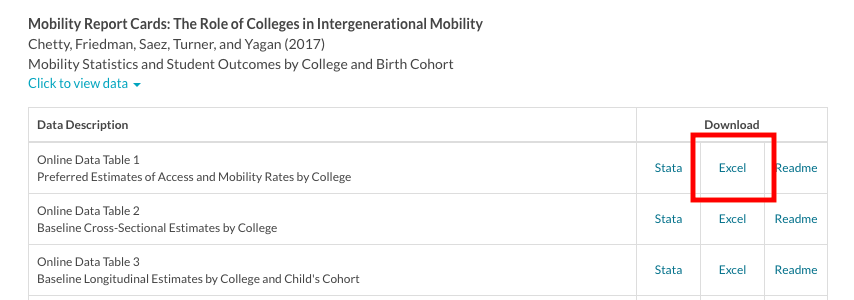
\includegraphics{~/Desktop/GitHub/rclass/lectures/lecture8/mrc_table1.png}~

\end{frame}

\begin{frame}[fragile]{Downloading data from web}

{[}FIX OUTPUT (CUTTING OFF){]}

\begin{Shaded}
\begin{Highlighting}[]
\CommentTok{#Paste url to excel "csv" file}
\NormalTok{data_url <-}\StringTok{ "http://www.equality-of-opportunity.org/data/college/mrc_table1.csv"}

\CommentTok{#Download data and read in using read_csv (readr)}
\NormalTok{mrc <-}\StringTok{ }\KeywordTok{read_csv}\NormalTok{(data_url)}

\CommentTok{#View first 4 rows and 4 columns }
\NormalTok{mrc[}\DecValTok{1}\OperatorTok{:}\DecValTok{4}\NormalTok{, }\DecValTok{1}\OperatorTok{:}\DecValTok{4}\NormalTok{]}
\CommentTok{#> # A tibble: 4 x 4}
\CommentTok{#>   super_opeid                                         name   czname state}
\CommentTok{#>         <int>                                        <chr>    <chr> <chr>}
\CommentTok{#> 1        2665 Vaughn College Of Aeronautics And Technology New York    NY}
\CommentTok{#> 2        7273               CUNY Bernard M. Baruch College New York    NY}
\CommentTok{#> 3        2688              City College Of New York - CUNY New York    NY}
\CommentTok{#> 4        7022                          CUNY Lehman College New York    NY}
\end{Highlighting}
\end{Shaded}

\end{frame}

\begin{frame}[fragile]{Downloading data from web}

Alternative approach

\begin{Shaded}
\begin{Highlighting}[]
\CommentTok{#Download data and read in link directly using read_csv (readr)}
\NormalTok{mrc <-}\StringTok{ }\KeywordTok{read_csv}\NormalTok{(}\StringTok{"http://www.equality-of-opportunity.org/data/college/mrc_table1.csv"}\NormalTok{)}
\CommentTok{#> Parsed with column specification:}
\CommentTok{#> cols(}
\CommentTok{#>   super_opeid = col_integer(),}
\CommentTok{#>   name = col_character(),}
\CommentTok{#>   czname = col_character(),}
\CommentTok{#>   state = col_character(),}
\CommentTok{#>   par_median = col_integer(),}
\CommentTok{#>   k_median = col_integer(),}
\CommentTok{#>   par_q1 = col_double(),}
\CommentTok{#>   par_top1pc = col_double(),}
\CommentTok{#>   kq5_cond_parq1 = col_double(),}
\CommentTok{#>   ktop1pc_cond_parq1 = col_double(),}
\CommentTok{#>   mr_kq5_pq1 = col_double(),}
\CommentTok{#>   mr_ktop1_pq1 = col_double(),}
\CommentTok{#>   trend_parq1 = col_double(),}
\CommentTok{#>   trend_bottom40 = col_double(),}
\CommentTok{#>   count = col_double()}
\CommentTok{#> )}
\end{Highlighting}
\end{Shaded}

\end{frame}

\begin{frame}[fragile]{Downloading data from web}

\begin{Shaded}
\begin{Highlighting}[]
\CommentTok{#View first 4 rows and 4 columns }
\NormalTok{mrc[}\DecValTok{1}\OperatorTok{:}\DecValTok{4}\NormalTok{, }\DecValTok{1}\OperatorTok{:}\DecValTok{4}\NormalTok{]}
\CommentTok{#> # A tibble: 4 x 4}
\CommentTok{#>   super_opeid                                         name   czname state}
\CommentTok{#>         <int>                                        <chr>    <chr> <chr>}
\CommentTok{#> 1        2665 Vaughn College Of Aeronautics And Technology New York    NY}
\CommentTok{#> 2        7273               CUNY Bernard M. Baruch College New York    NY}
\CommentTok{#> 3        2688              City College Of New York - CUNY New York    NY}
\CommentTok{#> 4        7022                          CUNY Lehman College New York    NY}
\end{Highlighting}
\end{Shaded}

\end{frame}

\begin{frame}{Problems downloading data (zip files) using IPEDS}

\begin{enumerate}
\def\labelenumi{\arabic{enumi}.}
\tightlist
\item
  Follow this \href{https://nces.ed.gov/ipeds/use-the-data}{link} and
  under the ``Survey Data'' tab select ``Complete data files''.\\
\item
  Choose ``All years'' and ``All surveys'' and click continue\\
\item
  Right click and copy link address for ``IC2017\_AY''
\end{enumerate}

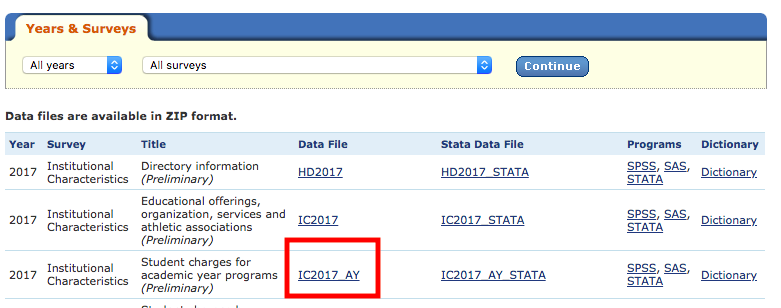
\includegraphics{~/Desktop/GitHub/rclass/lectures/lecture8/ic2017_ay.png}~

\end{frame}

\begin{frame}[fragile]{Downloading data (zip files) using IPEDS}

Paste url and read in using \texttt{read\_csv}\\
What happens when you try reading in this zip file?\\
Need to download \textbf{and} unzip

\end{frame}

\begin{frame}[fragile]{Downloading data (zip files) using IPEDS}

\begin{Shaded}
\begin{Highlighting}[]
\CommentTok{#Set path to where data will be saved}
\KeywordTok{setwd}\NormalTok{(}\StringTok{"~/Desktop/lecture8"}\NormalTok{)}
\CommentTok{#download file and pa}
\KeywordTok{download.file}\NormalTok{(}\StringTok{"https://nces.ed.gov/ipeds/datacenter/data/IC2017_AY.zip"}\NormalTok{,}
              \DataTypeTok{destfile =} \StringTok{"ic2017_ay"}\NormalTok{, }\DataTypeTok{mode =} \StringTok{'wb'}\NormalTok{)}
\CommentTok{#unzip zip file and keep original name}
\KeywordTok{unzip}\NormalTok{(}\DataTypeTok{zipfile =} \StringTok{"ic2017_ay"}\NormalTok{ , }\DataTypeTok{unzip =} \StringTok{"unzip"}\NormalTok{)}
\CommentTok{#> arguments 'minimized' and 'invisible' are for Windows only}

\NormalTok{ic2017_ay <-}\StringTok{ }\KeywordTok{read_csv}\NormalTok{(}\StringTok{"ic2017_ay.csv"}\NormalTok{)}
\CommentTok{#> Parsed with column specification:}
\CommentTok{#> cols(}
\CommentTok{#>   .default = col_character(),}
\CommentTok{#>   UNITID = col_integer()}
\CommentTok{#> )}
\CommentTok{#> See spec(...) for full column specifications.}
\end{Highlighting}
\end{Shaded}

\end{frame}

\begin{frame}{Student exercise}

\textbf{Tying it all together}

\begin{itemize}
\tightlist
\item
  Using everything we learned today read in a csv data file from the
  web\\
\item
  Go back to the ipeds data center
  \href{https://nces.ed.gov/ipeds/datacenter/DataFiles.aspx}{here}\\
\item
  Right click and copy the link address to a different data file
  (``HD2017'', ``EFFY2017'')\\
\item
  Make sure to download the link first (download.file) before reading
  in\\
\item
  Change column names to lowercase
\item
  Report dimensions of data\\
\item
  Create a subset of your data (filter, select, etc.)
\end{itemize}

\end{frame}

\section{Data sources (maybe)}\label{data-sources-maybe}

\end{document}
